\documentclass[letterpaper,11pt]{article}
\usepackage[english]{babel}
\usepackage[utf8]{inputenc}
\usepackage[nottoc]{tocbibind}
\usepackage[margin=1.25in]{geometry}
\usepackage[activate={true,nocompatibility},final,
			tracking=true,kerning=true,spacing=true,
			factor=1100,stretch=10,shrink=10]{microtype}

\usepackage{amsmath,apacite,graphicx,wrapfig,setspace,tikz,pgfplots,booktabs}
\usepackage[justification=centering]{caption}
\usetikzlibrary{matrix,arrows,calc,3d,fit,patterns}
\frenchspacing

\title{A Universal Robotic Control System using Reinforcement Learning with Limited Feedback}

\author{Joshua Gruenstein \and Michael Truell}

\begin{document}

\maketitle


% 100-200 words

\begin{abstract}

A robot control system was developed that could be taught tasks through reinforcement learning.  The system, nicknamed Fido, was designed to be universal regardless of the specific hardware inputs and outputs, and does not need to be modified for the task at hand.  This was achieved through the training of artificial neural networks coupled with a wire-fitted moving least squares interpolator following the $Q$-learning reinforcement algorithm.  A kinematically accurate robot was simulated with a differential drive system, a sensor array, and other outputs.  The robot was successfully trained to do an array of tasks with limited feedback iterations, such as following a radio emitter and blinking a multicolor light-emitting diode.

\end{abstract}


\pagebreak

\section{Introduction}

The most prevalent control system used in mobile robotics is a procedurally programmed expert system (Biggs \& MacDonald, 2003).  Such systems use linear conditional logic in order to emulate a desired behavior.  However, such systems are limited in numerous respects.  First, they can only perform the specific task for which they were programmed to accomplish; the entire software must be rewritten in order to change the target task.  Second, they rely on a knowledge of the inputs and outputs to the robot (such as sensors and motor control) in order to function.  The purpose of Fido was to solve both of these problems, allowing a universal general control system for robots that can be trained on tasks using reinforcement learning.

We chose to approach this problem with artificial neural networks; function appropriators modeled after nature with the capability to take in a large number of inputs to produce an output.  Neural networks are commonly used to solve tasks that are challenging using traditional rule-based programming, making them perfect for our task.  The control system was named Fido for the name's connotations to training an intelligent organism. 

\section{Neural Network Background}

\subsection{Neuron Architecture}

\begin{figure}
	\centering
	\def\layersep{2.5cm}
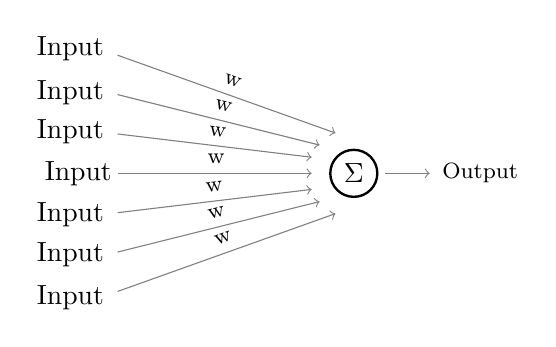
\begin{tikzpicture}[shorten >=1pt,->,draw=black!50, node distance=\layersep]
    \tikzstyle{every pin edge}=[<-,shorten <=1pt]
    \tikzstyle{neuron}=[circle,line width=0.3mm,draw=black,minimum size=17pt,inner sep=0pt]
    \tikzstyle{annot} = [text width=4em, text centered]


    \draw[->] (-3,1.5) -- (-.2,.5) node[sloped,midway,above] {\footnotesize w} node[left=3.4cm,above=.8cm]{Input};
    \draw[->] (-3,1) -- (-.4,.35) node[sloped,midway,above] {\footnotesize w} node[left=3.2cm,above=.4cm]{Input};
    \draw[->] (-3,0.5) -- (-.5,.2) node[sloped,midway,above] {\footnotesize w} node[left=3.1cm,above=.05cm]{Input};
    \draw[->] (-3,0) -- (-.5,0) node[sloped,midway,above] {\footnotesize w} node[left=2.45cm]{Input};
    \draw[->] (-3,-0.5) -- (-.5,-.2) node[sloped,midway,above] {\footnotesize w} node[left=3.1cm,below=.05cm]{Input};
    \draw[->] (-3,-1) -- (-.4,-.35) node[sloped,midway,above] {\footnotesize w} node[left=3.2cm,below=.4cm]{Input};
    \draw[->] (-3,-1.5) -- (-.2,-.5) node[sloped,midway,above] {\footnotesize w} node[left=3.4cm,below=.8cm]{Input};
    
    \node[neuron] (0,0) {$\Sigma$};

    \draw[->] (.4,0) -- (1,0) node[right] {\footnotesize Output};
\end{tikzpicture}
	\caption{Single Neuron Diagram}
\end{figure}

\begin{figure}[ht]
	\centering
	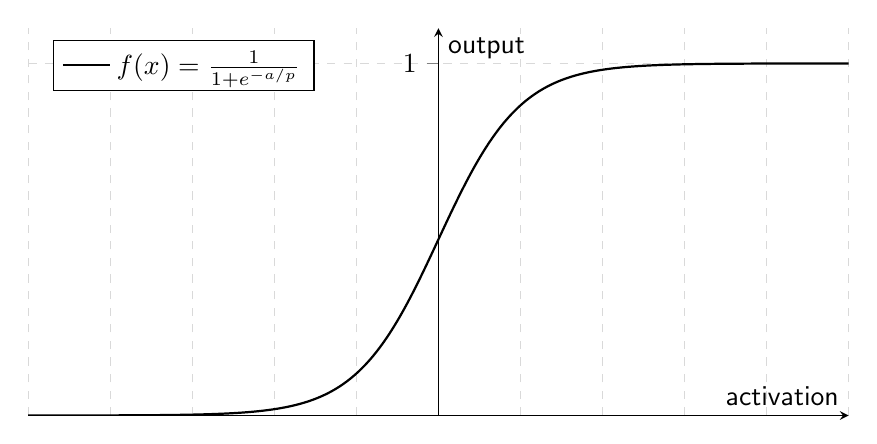
\begin{tikzpicture}[font=\sffamily]
    \begin{axis}[
    	legend pos=north west,
        axis x line=middle,
        axis y line=middle,
        grid = major,
        width=12cm,
        height=6.5cm,
        grid style={dashed, gray!30},
        xmin=-1,xmax= 1,ymin= 0,ymax= 1.1,
        xlabel=activation,ylabel=output,
        tick align=outside,
        ytick={1},
        xmajorticks=false,
        enlargelimits=false]
      \addplot[domain=-1:1,black,thick,samples=500] {1/(1+exp(-10*x))}; 
      \addlegendentry{$f(x)=\frac{1}{1+e^{-a/p}}$}
    \end{axis} 
\end{tikzpicture}
	\caption{Sigmoid Function Graph}
\end{figure}

\begin{figure}[ht]
	\centering
	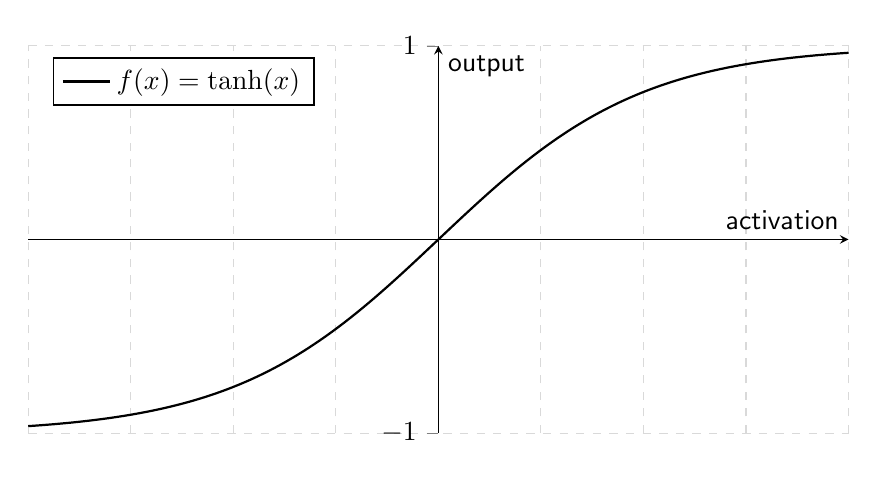
\begin{tikzpicture}[font=\sffamily]
    \begin{axis}[
    	legend pos=north west,
        axis x line=middle,
        axis y line=middle,
        grid = major,
        width=12cm,
        height=6.5cm,
        grid style={dashed, gray!30},
        xmin=-2,xmax= 2,ymin= -1,ymax= 1,
        xlabel=activation,ylabel=output,
        tick align=outside,
        ytick={-1,1},
        xmajorticks=false,
        enlargelimits=false]
      \addplot[domain=-2:2,black,thick,samples=500] {tanh(x)}; 
      \addlegendentry{$f(x)=\tanh(x)$}
    \end{axis} 
\end{tikzpicture}
	\caption{Hyperbolic Tangent Function Graph}
\end{figure}

\subsection{Feedforward Neural Network}

\begin{figure}[ht]
	\centering
	\def\layersep{2.5cm}
\begin{tikzpicture}[shorten >=1pt,->,draw=black!50, node distance=\layersep,font=\sffamily]
    \tikzstyle{every pin edge}=[<-,shorten <=1pt]
    \tikzstyle{neuron}=[circle,line width=0.3mm,draw=black,minimum size=17pt,inner sep=0pt]
    \tikzstyle{annot} = [text width=4em, text centered]

    \foreach \name / \y in {1,...,4}
        \node[neuron, pin=left:Input \y] (I-\name) at (0,-\y) {};

    \foreach \name / \y in {1,...,5}
        \path[yshift=0.5cm]
            node[neuron] (H-\name) at (\layersep,-\y cm) {};

    \node[neuron,pin={[pin edge={->}]right:Output}, right of=H-3] (O) {};

    \foreach \source in {1,...,4}
        \foreach \dest in {1,...,5}
            \path (I-\source) edge (H-\dest);

    \foreach \source in {1,...,5}
        \path (H-\source) edge (O);

    %\draw[->] (5,-2.9) -- (5,-5) -- (1,-5) -- (1,-4.5);
    %\node (1,-4.5) {Error back propagation}

    \node[annot,above of=H-1, node distance=1cm] (hl) {Hidden layer};
    \node[annot,left of=hl] {Input layer};
    \node[annot,right of=hl] {Output layer};
\end{tikzpicture}
	\caption{Single Output Feedforward Network}
\end{figure}

\section{Learning Implementation}

% Intro text here; a sentence or two
Intro text.

\subsection{Q-Learning}

Reinforcement learning seeks to find the optimal action to be undertaken for a given state through trial and error. In the context of Fido, an action can be the playing of a note or driving straight forward, and the state can be the amount of light detected by the robot or how near the robot is to another object. Once an action is performed, a reward and a new state are given back to the reinforcement learning algorithm. Overtime as actions are performed, a reinforcement learning algorithm sharpens its ability to receive reward.

Q-Learning (Watkins, 1989) is a popular reinforcement learning algorithm that works by learning an action-value function that takes an action-state pair as an input and outputs an expected utility value of performing that action in that state. This utility value is know as the $Q$-value. The $Q$-value is a combination of immediate reward and expected future reward. Every reward iteration, the $Q$-value of an action-state pair is updated as such:

\begin{equation}
	Q(a, s) := Q(a, s)(1 - \alpha) + \alpha(R + \gamma \max Q(a, s_{t+1}))
	\,,
\end{equation}

Where $a$ is the action carried out, $s$ is the initial state, $R$ is the reward received, and $s_{t+1}$ is the new state. $\alpha$ is the learning rate of the algorithm. $\alpha$ determines the rate of convergence by diminishing or amplifying the changes made to the $Q$-value each reward iteration. $\gamma$ is the devaluation factor, which determines the weight given to future rewards. A $\gamma$ approaching zero will force the algorithm to only value immediate reward, while a $\gamma$ approaching one will make it focused on high long term reward.

\subsection{Wire-Fitted Q-Learning}


\section{Simulation}

The robot model chosen for simulation was modeled after easily producible robots on the same scale.  The software driving the simulation was intended to be portable enough to work on a hardware implementation, and the model facilitates this goal as well.  Additionally, the robot model would have to be easily trainable and debuggable when implemented in hardware; use of a Geiger counter as an input would be unfavorable.  Lastly the sensors and design chosen had to facilitate the concept of natural learning, modeling after nature to some degree.

\subsection{Robot Inputs and Outputs}

Multiple inputs were modeled for simulation with outlets for control both by a human operator using sliders and by programmed handlers using a bridge class.  A microphone and light sensor were chosen as clear, human modifiable inputs that model after nature and could easily be used for reinforcement training.  An infrared light sensor was added as another easily controller variable in a testing setup: a human operator could easily bring closer and farther an IR LED for purposes of training.   Additionally sensors for battery level, three axes of accelerometers, and three axes of gyroscopes were added as more complex inputs for Fido to master.  


\subsection{Implementation and Kinematics}

\section{Results}

Results, testing, and applications go here.
\long\def\/*#1*/{}
\subsection{Training Methods}

\subsection{Findings}

\begin{figure}[ht]
	\centering
	\footnotesize
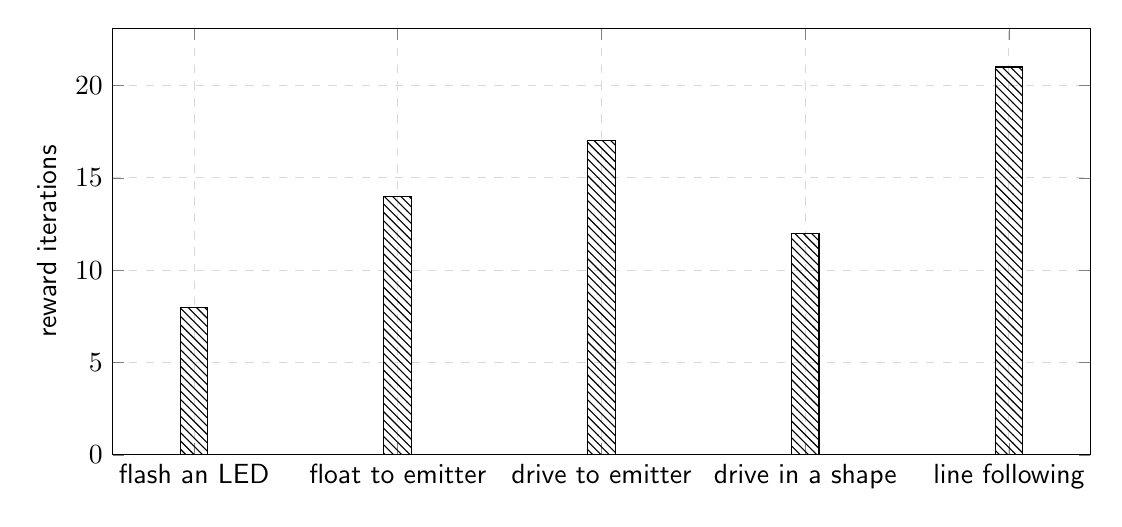
\begin{tikzpicture}[font=\sffamily]
\begin{axis}[
    	symbolic x coords={flash an LED,
                           float to emitter,
    					   drive to emitter,
    					   drive in a shape,
    					   line following},
    	ylabel={reward iterations},
    	width = 14cm, height = 7cm,
        grid=major,grid style={dashed, gray!30},
        ymin=0,xtick=data]
    
    \addplot[ybar,pattern=north west lines] coordinates {
        (flash an LED,8)
        (float to emitter,14)
        (drive to emitter,17)
        (drive in a shape,12)
        (line following, 21)
    };
\end{axis}
\end{tikzpicture}
	\caption{Number of Reward Iterations for Fido Learning Tasks}
\end{figure}

\begin{figure}[ht]
	\centering
	\footnotesize
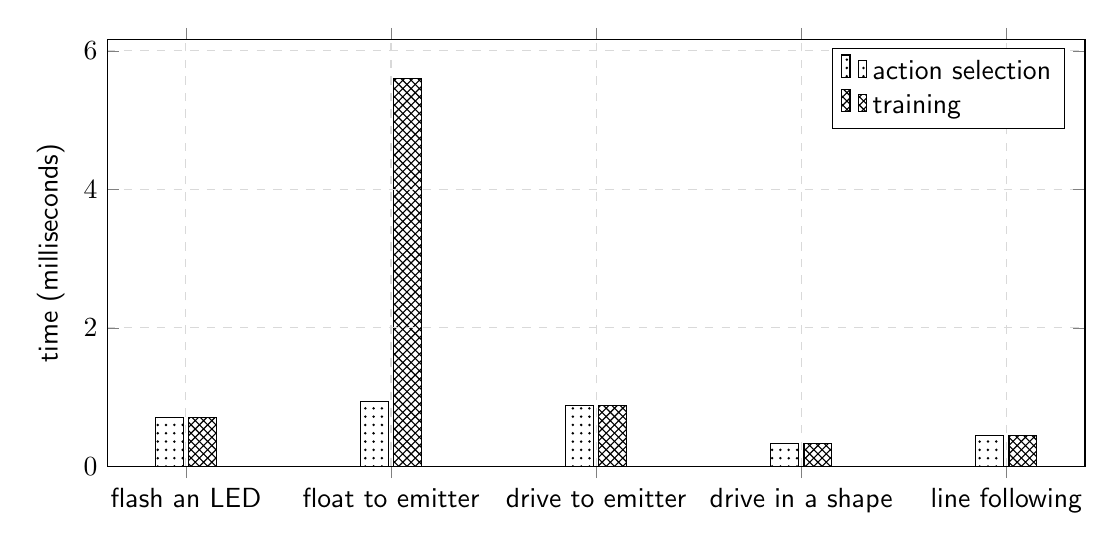
\begin{tikzpicture}[font=\sffamily]
    \begin{axis}[
        legend cell align=left,ybar=2pt,
        bar width=10pt,ymin=0,axis on top,
        xtick=data,ylabel=time (milliseconds),
        grid=major,grid style={dashed, gray!30},
        symbolic x coords={flash an LED,float to emitter,
                           drive to emitter,drive in a shape,
                           line following},
        xmin={flash an LED},xmax={line following},
        enlarge x limits={abs=1cm},
        width=14cm,height = 7cm
    ]

        \addplot[pattern=dots] coordinates {
            (flash an LED,0.7)
            (float to emitter,0.94)
            (drive to emitter,0.88)
            (drive in a shape, 0.33)
            (line following, 0.45)
        };

        \addplot[pattern=crosshatch] coordinates {
            (flash an LED,0.7)
            (float to emitter,5.6)
            (drive to emitter,0.88)
            (drive in a shape, 0.33)
            (line following, 0.45)
        };

        \legend{action selection,training};
    \end{axis}
\end{tikzpicture}

	\caption{Time to Learn for Fido Learning Tasks}
\end{figure}

\/*
Outline
- Compare to discrete
- Compare to other action selection methods
- Compare to actor critic

*/

\subsection{Further Applications}

\section{Discussion}

\subsection{Software Plans}

Currently, the number of wires that our neural network outputs is constant. However, the complexity of the functions that the wire-fitting function has to model varies from task to task. To add to the portability of Fido, we plan on implementing a method of dynamically changing the number of wires that the neural network outputs. Such a method would gage the variance and bias that the interpolator is experiencing. Variance is the deviation of a function from its mean. The wire-fitting function's variance could be measured in a range of actions. Bias is the error that results from under fitting, and could be measured as the moving average of the wire-fitted interpolator function's error at predicting Q-values, or the moving average of the distance that the wire-fitting function's wires have to move during gradient descent. Our proposed method would use $bias^2 + variance$ as a cost function and would look to reduce its by testing changes to the number of wires to determine the direction of the cost function. Each time a wire is removed or added to create a new set of wires, this set of wires will be changed to best model the wire-fitting function formed by the past set of wires.

The topology of our feedforward neural networks is static throughout Fido's lifetime. To increase the generality of Fido, we would like to research ways to evolve the topology of Fido's neural network as performs action and receives reward. This may mean measuring variance and bias values and determining the direction of $bias^2 + variance$ as outlined above, but may also take the form of an existing variation of back propagation, of which there are many.

\subsection{Hardware Implementation}

\section{Conclusion}

A general robotic control system nicknamed Fido was developed that learned tasks with limited feed back. Fido couple the training of artificial neural networks with a wire-fitted moving least squares interpolator to achieve a continuous state-action space $Q$-learning reinforcement algorithm implementation. Fido leveraged a Boltzmann distribution of probability based on reward to select actions, allowing it to continuously explore its state-action space. A kinematically accurate robot was simulated with a differential drive system, a sensor array, and other outputs to test Fido. The robot was trained on a number of common robotic tasks and successfully converged on these tasks in less reward iterations than all other actors tested, while maintaining impressively low latency. In the future, we hope to improve Fido's software further and are working toward the completion of Fido's hardware implementation.

\nocite{gaskett,geoffrey,werbos,dini,macleod,dongsoo,dudek,watkins,rummery,baird}

\pagebreak
\bibliography{Paper}
\bibliographystyle{apacite}

\end{document}